\documentclass[]{asaproc}\usepackage[]{graphicx}\usepackage[]{color}
%% maxwidth is the original width if it is less than linewidth
%% otherwise use linewidth (to make sure the graphics do not exceed the margin)
\makeatletter
\def\maxwidth{ %
  \ifdim\Gin@nat@width>\linewidth
    \linewidth
  \else
    \Gin@nat@width
  \fi
}
\makeatother

\definecolor{fgcolor}{rgb}{0.345, 0.345, 0.345}
\newcommand{\hlnum}[1]{\textcolor[rgb]{0.686,0.059,0.569}{#1}}%
\newcommand{\hlstr}[1]{\textcolor[rgb]{0.192,0.494,0.8}{#1}}%
\newcommand{\hlcom}[1]{\textcolor[rgb]{0.678,0.584,0.686}{\textit{#1}}}%
\newcommand{\hlopt}[1]{\textcolor[rgb]{0,0,0}{#1}}%
\newcommand{\hlstd}[1]{\textcolor[rgb]{0.345,0.345,0.345}{#1}}%
\newcommand{\hlkwa}[1]{\textcolor[rgb]{0.161,0.373,0.58}{\textbf{#1}}}%
\newcommand{\hlkwb}[1]{\textcolor[rgb]{0.69,0.353,0.396}{#1}}%
\newcommand{\hlkwc}[1]{\textcolor[rgb]{0.333,0.667,0.333}{#1}}%
\newcommand{\hlkwd}[1]{\textcolor[rgb]{0.737,0.353,0.396}{\textbf{#1}}}%
\let\hlipl\hlkwb

\usepackage{framed}
\makeatletter
\newenvironment{kframe}{%
 \def\at@end@of@kframe{}%
 \ifinner\ifhmode%
  \def\at@end@of@kframe{\end{minipage}}%
  \begin{minipage}{\columnwidth}%
 \fi\fi%
 \def\FrameCommand##1{\hskip\@totalleftmargin \hskip-\fboxsep
 \colorbox{shadecolor}{##1}\hskip-\fboxsep
     % There is no \\@totalrightmargin, so:
     \hskip-\linewidth \hskip-\@totalleftmargin \hskip\columnwidth}%
 \MakeFramed {\advance\hsize-\width
   \@totalleftmargin\z@ \linewidth\hsize
   \@setminipage}}%
 {\par\unskip\endMakeFramed%
 \at@end@of@kframe}
\makeatother

\definecolor{shadecolor}{rgb}{.97, .97, .97}
\definecolor{messagecolor}{rgb}{0, 0, 0}
\definecolor{warningcolor}{rgb}{1, 0, 1}
\definecolor{errorcolor}{rgb}{1, 0, 0}
\newenvironment{knitrout}{}{} % an empty environment to be redefined in TeX

\usepackage{alltt}
\usepackage{amsmath}
%\usepackage{mathtools}
%\usepackage{breqn}
\usepackage[title]{appendix}

% Image
\usepackage{graphicx}
\graphicspath{ {./figures/} }
\usepackage{subcaption}
%\usepackage[utf8]{inputenc}
\usepackage[export]{adjustbox}
\usepackage{wrapfig}
\usepackage{float}

%Table
\usepackage{array}
%\usepackage{longtable}
%\usepackage[table]{xcolor}
\usepackage{verbatim}

%\usepackage[english]{babel}

%\usepackage{times}
%If you have times installed on your system, please
%uncomment the line above

%For figures and tables to stretch across two columns
%use \begin{figure*} \end{figure*} and
%\begin{table*}\end{table*}
% please place figures & tables as close as possible
% to text references

% Save output to txt
%sink("summary.txt")
%summary(fit1)
%sink(NULL)

%\newcommand{\be}{\begin{equation}}
%\newcommand{\ee}{\end{equation}}

\title{Using Linear Models to Analyze Returns in Pop Art}

%input all authors' names

\author{Brewer Cappellin, A$^1$, Coleman, A$^1$\\
Department of Statistics, University of California at Santa Cruz$^1$\\}

%input affiliations

%{USDA Forest Service Forest Products Laboratory}
\IfFileExists{upquote.sty}{\usepackage{upquote}}{}
\begin{document}
%\SweaveOpts{concordance=TRUE}

\maketitle



















\begin{abstract}
For this project, we investigated the performance of Pop Art as an investment by exploring the meaningful characteristics that determine the price of an artwork. We performed a linear regression analysis using log of price as our response variable and ten predictors that uniquely describe each piece of art. We created a market price index to show the variations of Pop Art over the 2001-2012 period when considering the regression coefficients from the predictor ``year'' as a factor. Our price index results showed that during this period, the Pop Art market appreciated by $5.52$\% on average per year in real USD while our benchmark, the index for the S\&P 500 (S\&P), barely depreciated by $0.01$\% on average per year in real USD. These results showed that investing in Pop Art, during this time period, provides a higher return than investing in the stock market or low-risk corporate bonds.
\begin{keywords}
pop art, linear regression, price analysis, linear models, investments, price index
\end{keywords}
\end{abstract}

\section{Introduction}

Over the last several decades, news stories containing accounts of fine art selling for staggering amounts of money continue to astound the public. We can see many of these notable instances in just the last decade of the Pop Art Movement. In January 2017, a work titled ``Masterpiece'' by Roy Lichtenstein sold for \$165 million. In November 2015, another Lichtenstein piece titled ``Nurse'' sold for \$95.4 million. In May 2015, an untitled artwork by Jean-Michel Basquiat sold for  \$110.5 million. In March 2010, a Jasper Jhones piece was sold for \$110 million. Finally, in October 2008, an Andy Warhol piece titled ``Eight Elvis'' sold for \$100 million. All of the aforementioned famous artists are included in our dataset along with many other artists whose art does not exceed the multimillion-dollar mark.

The growth of these multimillion dollar sales, the expansion of high-net-worth individuals, and the need for portfolio diversification in recent years have commanded a lot of attention to the art investment world. However, these high prices should not necessarily imply high returns for investments.

In order to assess the return on investment for the Pop Art market during this time period, we will perform a multiple regression analysis that will use price as our response and other variables as predictors. To select these other variables, we will execute in-depth exploratory data analysis (EDA). We will then build our model from these predictors. Finally, we will divide our complete data set into a training and test set to assess the predictive capability of our model. 

As a comparison to our first model, we will remove the high-value artworks from our dataset and fit a second model to see if removing these large observations improves the predictive power of our model.


\subsection{Prior Analysis}

Two papers helped to influence our methods and analysis. 
The first paper, from Mei J, Moses M (1), did a similar analysis with artworks ranging from 1875 to 1999. They performed multiple linear regression on the data and calculated the returns. Their work concluded a real return of 4.9\% per year and a higher rate of 8.2\% per year after 1950. The second paper, Renneboog L, Spaenjers C (2), created an index for a database of over 1,000,000 artworks across multiple art movements sold from 1957 to 2007. Their result showS that art appreciated in value by 3.97\% per year in real USD; a trend similar to that of corporate bonds.

With these two papers in mind, we performed an analysis only focused on the Pop Art movement while in a turbulent period for the stock market. Between the years 2000 and 2012, we had two important market crashes: the dot-com crash in 2000 and the Financial Crisis of 2007. This time period provided an interesting data set while also creating difficulties that we will explore in later sections. 

\section{Data}

We are using a data set comprised of multiple art movements obtained from a web scrape conducted over the course of six months. Using the complete data set would be far outside the scope for this project. Therefore, we will be doing our analysis on a subset of this data set: the Pop Art Movement. With this subset, our data consists of 27,124 observations; having over 20 variables that contain characteristics of the art and sale information from 2000 to 2012.

To help reduce and understand the myriad of potential variables for our model, we referenced Renneboog L, Spaenjers C (2). When trying to predict the price of an artwork, we see that our variables can be classified under the categories shown in Table \ref{att}.


\begin{table}[H]
\caption{\enspace Variables}\label{att}
\begin{tabular*}{\hsize}{@{\extracolsep{\fill}}ccc}
\\[-5pt]
\multicolumn{1}{c}{\it Sale attributes} & 
\multicolumn{1}{c}{\it Artwork attributes} & 
\multicolumn{1}{c}{\it Artist attributes}\\
\hline
\\[-5pt]
Price & Material & Name \\
Auction house & Signed & Origin\\
Location sold & Dated & Vital status\\ 
Year sold & Area & \\ 
Month sold &  & \\ 
\hline
\end{tabular*}
\end{table}

%\emph{Artist traits}: name, origin, and vital status
%\emph{Artwork characteristics}: material, area of the artwork in square inches, signed, and dated
%\emph{Sale information}: price, month sold, year sold, auction house, and auction house location

\subsection{Data Manipulation}

Before fitting a model, extensive data manipulation is needed. First, we removed all duplicate entries in our data. Using web scraping as a data collection method, we obtained $103$ duplicate sale entries. 

Next, we want to make sure that our data are aptly prepared to create a price index. For this index, we need to remove data from incomplete years. After removing the partial data from 2013, we are left with our final data set that contains $25572$ observations.

Finally, we needed to check the proportion of repeated sales in our data set. Unfortunately, we found $3462$ repeated sales; roughly $13$\% of out total observations. Because of this artifact, we no longer can assume that our errors are independent. We continue with the analysis while keeping in mind that this might affect fitting our model as well as our results.

Now that we have established a final dataset, we corrected the prices for inflation. Our prices must represent real values from their respective time period. We selected the latest date of the works sold and proceeded to correct all of the prices to real values.

\subsection{Exploratory Data Analysis}

After our data manipulation, we performed exploratory data analysis to help understand our variables while assessing the usefulness of any transformed variables. As a baseline, we initially fitted a model with the data, without any transformations, and found that the errors were not $NID(0,\sigma^2)$ with a constant variance. Therefore, we proceeded to apply a log transformation to both our two continuous variables: area and price. 

With our newly transformed data, we fit a base model that contained all of the variables mentioned in section 2. This model was unable to estimate the coefficients of the different origin variables. We deduced that issue resulted from collinearity between artist names and artist origins; creating redundant information in our model. Therefore, we made sure to remove the variable that was the least statistically significant when selecting on our final model.

We then created different box plots of our factors against our log of price to assess the behavior of our data. Compared to our plots without a transformation on price, these plots (with the log of price) greatly improved; moving our predictor variables closer to our assumption criterion. This helped solidify our decision to keep the log of price as the transformation for our response variable. 

Our next plot is the Log of Price vs the Log of Area shown in Figure \ref{area}. This plot depicts two different, unintentional clusters of artworks that may cause problems with the fit of our final model. In this plot, we see that the smaller cluster results from artworks that have an area of over 22,000 sq. inches. Compared to the bulk of our data, this small cluster is most likely a group of outliers and will create difficulties when making predictions with our final model.

The main group of points, centered around a price of \$22,000, similarly begins to disperse as the price of artwork increases. This dispersion will also cause problems with our model, especially concerning the prediction accuracy of high-valued art. As we will see in our later analysis with our final model, most of these artworks valued over \$350,000 will be underestimated.

\begin{figure}[H]

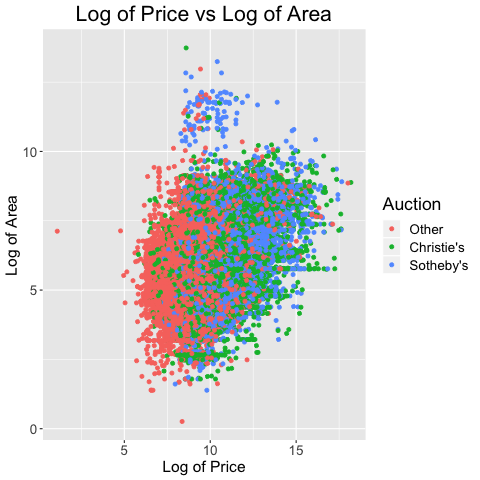
\includegraphics[scale = 0.5]{Area_SP}
\caption{Scatter plot of log of Price vs log of Price}
\label{area}
\end{figure}

For the final portion of our exploratory data analysis, we created dendrograms of our factor variables in an attempt to diminish the number of levels in both origins of artist and auction location. These dendrograms helped us decide where to cluster our different levels. 

In Figure \ref{origin_dendo} we can see how the clustering for the origin of the artist is dominated by Americans. We decided to group artist origin into two levels: ``American-British'' since the Pop Art Movement was predominantly an American-British movement, and ``Other''.

Regarding Figure \ref{place_dendo}, we similarly clustered the place of sale, but into three levels for ``New York'', ``London'', which includes South Kensington in it's larger metropolitan area, and ``Other''.

Like these two dendrograms shown below, we clustered auction houses as well and reducing the levels to the large auction houses of ``Sotheby's'' and ``Christie's'', then including the rest in ``Other''.

\begin{figure}[H]

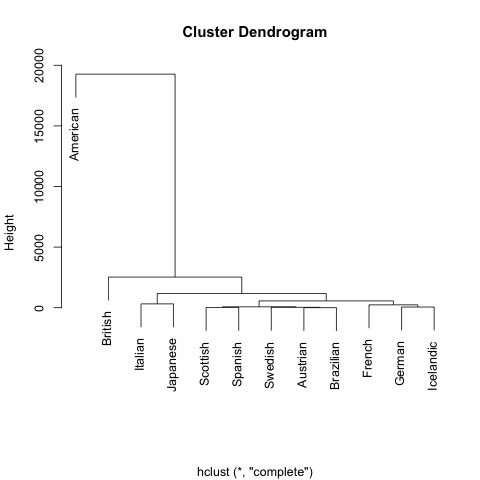
\includegraphics[scale = 0.5]{den1}
\caption{Dendogram for artist origin}
\label{origin_dendo}
\end{figure}

\begin{figure}[H]

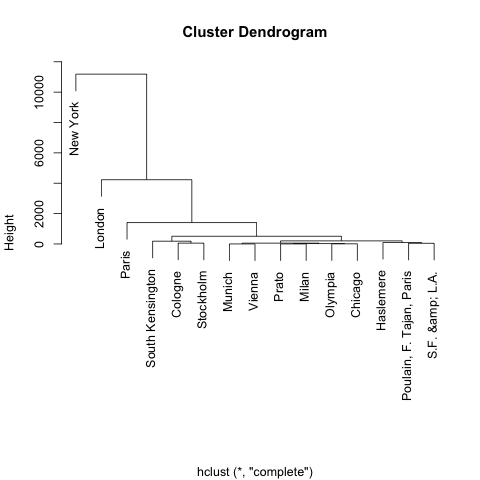
\includegraphics[scale = 0.5]{den2}
\caption{Dendogram for place of sale for the artwork}
\label{place_dendo}
\end{figure}

\section{Methods}

With our variables releveled, we can now begin to create a price index for the Pop Art Movement. We will use multiple linear regression to determine the value of the coefficients and the year variable to create the price index. We then use these index values to analyze returns per year. 
In addition to the construction of our price index, we will test the predictive power of our model. We will perform a 95:5 split of our data into a training and test set. Our training set will contain $24293$ observations and the test set will contain $1279$ observations.

\subsection{Model}

The equation of our model relates the log of the real price in USD to the year variable (factor), the log of the area (continuous), and the remaining variables that include artist traits, artworks characteristics, and sales information.

\footnotesize
\begin{align}
\ Ln(P_{k}) = \mu + \sum_{m=1}^M \beta_m X_{m,k} + \sum_{t=1}^T\gamma_t D_{t,k} + \alpha Ln(A_k) + \epsilon_{k} 
\label{model}
\end{align}
\normalsize

We see $P_{k}$ is the log of price of an artwork $k$, $X_{m,k}$ is the attribute $m$ (Table \ref{att}) of artwork $k$, $D_{t,k}$ is the year variable for artwork $k$ at year $t$ and $A_k$ is the variable for the log of area for each artwork $k$.

The coefficients $\beta_m$ relate to the attribute $m$, coefficient $\alpha$ related to the log of the area, and $\gamma_t$ are the coefficients for the year variable that will then be used to construct the price index for Pop Art.

The value of the index at year $t$ will be calculated using

\begin{align}
\Pi_t \equiv exp(\hat\gamma_t) \times 100 
\label{index_eq}
\end{align}

Where $\Pi_t$ is the value of the index at year $t$.

Because our initial year (2001) will be restricted as part of the intercept in our model, we must re-scale the year variable in order for it to be meaningful in the calculations of our index. This equation \ref{index_eq} provides us with the percentage growth for each year coefficient.

Silver M, Heravi S (3) provides us with an index that computes a geometric mean instead of an arithmetic mean. Because of the log transformation on the predictor variable, the geometric mean will be more useful in our case. Since the residuals for each year are normally distributed with constant variance, we corrected for the transformation bias using

\begin{align}
\Pi^*_t \equiv exp(\hat\gamma_t+\frac{1}{2}(\hat\sigma^2_t - \hat\sigma^2_{0}) \times 100
\label{corr_index}
\end{align}

where $\hat\sigma^2_{0}$ and $\hat\sigma^2_t$ are the estimated variances for the initial year (2001) and year t, respectively. Finally, we can calculate the estimated corrected returns for each year by

\begin{align}
r^*_t \equiv \frac{\Pi^*_t}{\Pi^*_{t-1}}-1 
\label{returns}
\end{align}

\subsection{Model Selection} 

With our model equation defined in equation \ref{model} and our transformed variables, we fit three different models in order to determine the most meaningful variables for a final model. Using this final model, we will then create our price index and make predictions. We know from our exploratory data analysis that the artist name and artist origin cannot be included in the same model due to collinearity. Therefore, we need to determine which of the two variable is the most successful in predicting the log of the price.

For our first model, we included only artist name along with our other variables. We took note of the model selection criterion AIC, BIC, and $R^2$ to help decide between contending models. 

Our second model removes the artist name and uses the origin variable with the rest of the variable. For this model, we also recorded our model selection criterion. 

Finally, our third potential model uses the artist name while removing the origin and location of sale. We wanted to determine if the sale location contributed any predictive power to our model.

In Table \ref{ABR} below, we summarized the model selection criteria for each of our three models. We see that by all three criterion, our first model performs the best. Therefore, we will keep our variables selected in section 2 and only remove artist origin in favor of artist name. 

\begin{table}[!ht]
\caption{\enspace AIC, BIC and $R^2$ for the three models fitted.}\label{ABR}
\begin{tabular*}{\hsize}{@{\extracolsep{\fill}}cccc}
\\[-5pt]
\multicolumn{1}{c}{\it Model} & 
\multicolumn{1}{c}{\it AIC} & 
\multicolumn{1}{c}{\it BIC} & 
\multicolumn{1}{c}{\it $R^2$}\\
\hline
\\[-5pt]
Model 1 & $73979$ & $74773$ & $0.5508$ \\ 
        Model 2 & $79720$ & $80020$ & $0.4282$ \\
        Model 3 & $74336$ & $75113$ & $0.5441$ \\
\hline
\end{tabular*}
\end{table} 

\subsection{Restrictions} 

We can see from our prior analysis and from Figure \ref{qq} that we have problems from heteroskedasticity (fat tails). Similarly, we know that not all of our necessary conditions are satisfied because of repeated sales: errors that are $NID(0,\sigma^2)$ with constant variance. Therefore, our model would need to be slightly changed or include different normalization of variables to achieve a better fit, which would be beyond the scope of this project. This restriction will thus affect our model fit and prediction accuracy.

\begin{figure}[!ht]

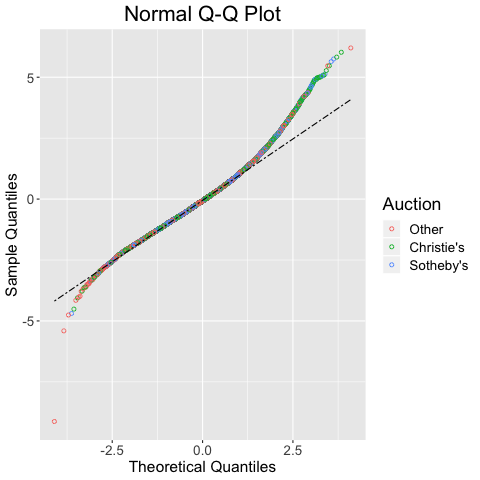
\includegraphics[scale = 0.5]{qq}
\caption{Normal Q-Q plot for Model 1, includes all original variables except origin of the artist}
\label{qq}
\end{figure}

\section{Results}

Table \ref{OLS} shows the estimates for all the parameters in our final model. In this case, equation \ref{model} is estimated using Ordinary Least Squares, where the dependent variable is the log of real prices in USD. Because the estimations have so many parameters, we will focus on their economic significance regarding their price prediction. The model sets restrictions to the following parameters by including them in the intercept: ``Andy Warhol'' for artist name, ``other'' for materials, ``other'' for auction house, ``other'' for locations, ``dead'' for vital status, ``none'' for signed, ``none'' for dated, ``2001'' for the year sold, and ``May'' for the month sold. 

To estimate the price impact of the parameters, we used the following equation

\begin{align}
Price\ Impact \equiv \exp(\hat\beta_m) - 1
\label{impact}
\end{align}

Where $\beta_m$ is the estimated coefficient for the parameter we want to analyze (Table \ref{OLS}).

The price analysis shows how the parameters impact the value of the artwork. Since our model was fitted with Andy Warhol as the baseline for artists, when considering only the impact of other artists, all of them have a negative impact on price except three that have non significant coefficients.

When we look at the materials, we can see that of other all the materials have a positive impact on the price artwork except prints when compared to our baseline. In the case of ``oil'' and ``acrylic'', we see that they have the highest price impact with $404.56$\% percent and $340.65$\% respectively.

If we compare the impact of the auction house and location of where the art was sold, we find a positive impact of the parameters over our baseline. Christie's has an positive price impact of $74.21$\% and Sotheby's of $77.83$\%. In the case of the place sold New York's price impact is $41.47$\% and London's is $69.49$\%.

As expected (because we did not include interaction effects), if the artist is alive at the time of the sale, we see a negative impact on the price. If the artwork is dated, it has a positive impact. On the other hand, a curious result from our regression model is that if the artwork is signed, it has a negative price impact of $-19.18$\%.

\begin{table}[H]
\caption{\enspace Ordinary Least Squares Estimates for our final model. The dependent variable is the log of price and the predictors are as mentioned in the model selection.}\label{OLS}
\tiny \verbatiminput{summary.txt}
\end{table}

\subsection{Index}

We can see the index we calculated for Pop Art alongside the index for the S\&P from 2001 to 2012 in Figure \ref{index_plot}. We used equation \ref{corr_index} to calculate the value of the Pop Art index and normalized both indices to start with an index value of 100 in 2001. For this comparison, we used the inflation-adjusted S\&P, obtained from Multpl.com (4). However, for a complete, comprehensive analysis, we needed to similarly adjust for inflation of the art prices before comparing to the S\&P index.  

It is clear that during this time period, the Pop Art market out-performed conventional investments, even when comparing returns to low-risk corporate bonds. Both markets suffered from high volatility due to the aforementioned crashes, but the Pop Art market was more robust than the traditional stock market. 
An interesting result from our analysis showed that the dot-com crash had a small impact compared to the later Financial Crisis.

Another noteworthy trend, displayed clearly in Figure \ref{index_plot}, shows a delay in the Pop Art market by about one year when compared directly to the stock market. This shows that people who invest in the Pop Art market have a slightly slower reaction time to alter their investments by about one year. This phenomenon can be explained by the time of the year in which large auctions occur. For example, in 2007, most of the sales closed before the bubble of the Financial Crisis burst, thus leaving the Pop Art market unaffected for that year, as seen below. 

\begin{figure}[!ht]

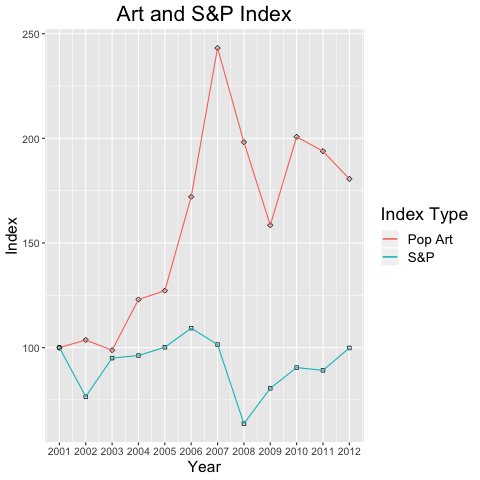
\includegraphics[scale = 0.5]{index}
\caption{Plot over time for Corrected index and S\&P}
\label{index_plot}
\end{figure}

Table \ref{return_table} allows us to analyze these results in much greater depth. During the aftermath of the dot-com crash, the Pop Art market remained mostly unaffected. However, the stock market suffered greater losses during the year 2002. Following this abysmal crash, both markets swiftly recovered; the stock market first by 2003 and then the Pop Art market by 2004. Later, leading up to the Financial Crisis, both markets suffered from high speculation, meaning that assets were continually purchased at higher and higher prices with the hope that their value will also increase in the near future.

We can see that the Pop Art market experienced more severe side effects from the crash by looking at the increase from 35.2\% to 41.3\% in 2006 and 2007 respectively. In the stock market, we only see an increase of 9.11\% in 2006 and then a gradual to a sharp decline by 2007. This led to a big crash for both markets following the bubble burst in 2008. We can see that the Pop Art market declined 18.5\% while the stock market decreased a staggering 37.2\%. This disconnect continues when in 2009, the Pop Art market remained in decline at a rate of 20.0\% while the stock market began its recovery at a rate of 26.5\%.
The Pop Art market did not begin to recover until the following year when returns in 2010 reached 26.6\%. For the final years of our time period, 2011 to 2012, we see that the stock market continued its recovery while the Pop Art market remained in decline. 

In conclusion, both markets suffered from high volatility during the period analyzed. However, despite this tumultuous time period, the Pop Art market clearly out-performed the stock market. Table \ref{return_table} summarizes the returns for both Pop Art and S\&P and also includes the Time Weighted Rate of Return (TWRR) over the 12 years period. We see that the Pop Art investments had an average return of $5.52$\% per year in real USD and the stock market returns were neutral at an average return of $-0.01$\% per year in real USD.

\begin{table}[!ht]
\caption{\enspace Returns for the S\&P and Pop Art by year. The last row shows the Time Weighted Rate of Return for each index.}\label{return_table}
\footnotesize \verbatiminput{returns.txt}
\end{table}

\subsection{Prediction}

We will now use the remaining 5\% of our data, preserved in a test set from our initial split, in order to assess our model's prediction capabilities. One method that we used to determine our model's predictive power was to compare the correlation between the actual values of the out of sample (test) data and the predicted values. We obtained a value of $0.75$, which indicates fair predictability for our model.

\begin{figure}[!ht]

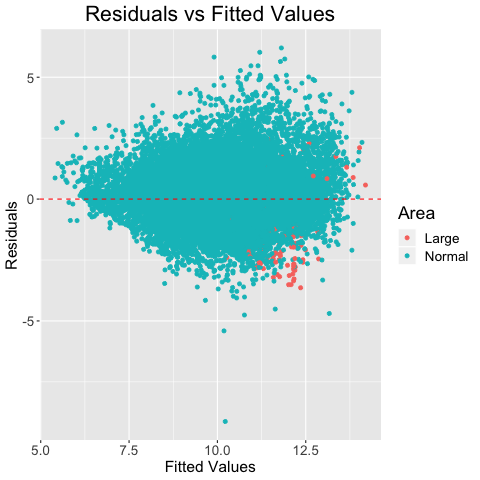
\includegraphics[scale = 0.5]{residuals}
\caption{Residual plot for Model 1 colored by Area Size, where large is an area over 22,000 sq. inches.}
\label{residuals}
\end{figure}

As another method of predicting accuracy is to compare the Mean Squared Errors (MSE). For the final model, we obtained $1.2255$ and for our out of sample MSE, we got $1.2657$. This small difference between both numbers ($3.28$\%) tells us that the out of sample prediction is performing similar to our final model.

As mentioned during EDA, the two different clusters that we observed in Figure \ref{area} might give problems for our predictions. Therefore Figure \ref{residuals} shows that the large artworks deviate in their residuals from the rest. It can be seen that the majority of the residuals are negative and far away from zero. This indicates that predictions for artworks with larger areas will not be as accurate. 

Figure \ref{pred} shows the residuals for the predicted values from the out of sample test data set. This plot has a clear pattern that confirms what was explored in the model restrictions. We can see that our model has issues predicting high-valued artworks: as the price of the art goes up, the residuals increase, telling us that the model is under predicting the value of these artworks. Similarly, we can also see that our model had difficulty predicting  for large area artworks, as hypothesized earlier. Here, most of our residuals fall below zero, indicating that the prices are mostly overpredicted.

\begin{figure}[!ht]

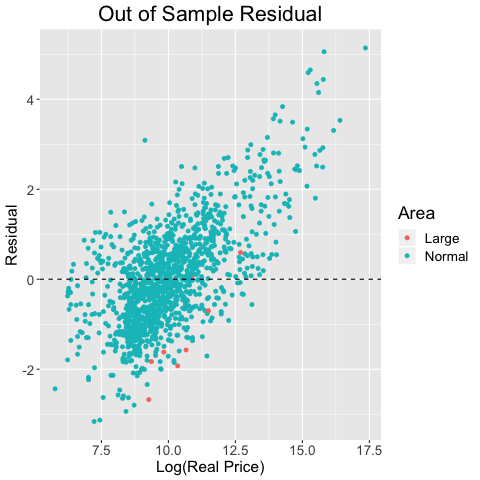
\includegraphics[scale = 0.5]{predict}
\caption{Plot of out of sample residual }
\label{pred}
\end{figure}

Given these egregious errors in prediction, we will introduce an additional model in the next section where we removed high valued artworks and compare the difference in indices, returns, and predictions.

\subsection{Additional Model}

Since our final model possesses issues predicting high-value artworks, we created an additional model using the same variables but with excluding the high-value artworks from our data. We will only include artworks below \$300,000. In total, $2012$ observations were removed, or approximately $7.87$\%  of the total data set.

Figure \ref{index_red_plot} compares both of the indices from the original model, with our whole data set, and this new model, using a subset of the data. As expected, both indices follow a very similar pattern, despite intersecting at various points in time. Most importantly, we observed no significant difference in the rate of returns. The original index had a  $5.52$\% average yearly return in USD and the reduced data set had $5.47$\% average yearly return in USD.
 
\begin{figure}[!ht]

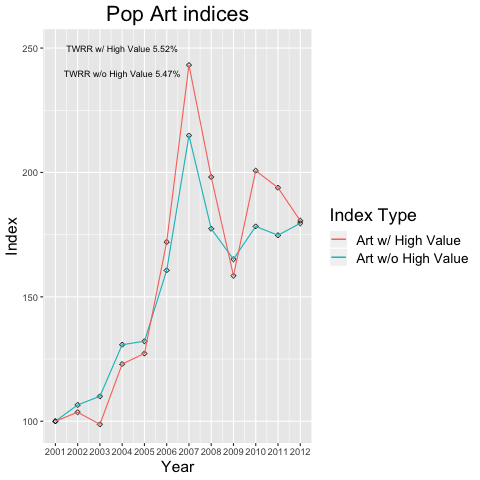
\includegraphics[scale = 0.5]{index_red}
\caption{Plot over time for the Pop Art index with and with out High Value artworks}
\label{index_red_plot}
\end{figure}

Given that the indices are almost identical, we must now decide whether the predictions made by our addition model exceed those made by our final model. We once again computed and compared the Mean Squared Error. We found that the in sample MSE for the additional model is $0.8474$ and the out of sample MSE is $0.8992$. The small difference between both numbers ($6.12$\%) tells us that the out of sample prediction is also performing well.

Figure \ref{pred_reduced} shows the out of sample residuals for our additional model. Unfortunately, we still are observing the same problem with accurately predicting prices for large artworks. However, we do see that are residuals and MSE are smaller as a direct result of removing high valued artworks. 

\begin{figure}[!ht]

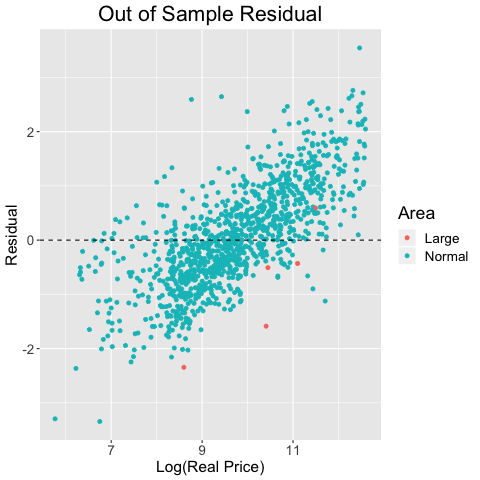
\includegraphics[scale = 0.5]{predict_red}
\caption{Plot of out of sample residual for data set with out High Value art}
\label{pred_reduced}
\end{figure}

Even though this additional model is incomplete in terms of developing a model for the entirety of Pop Art, we do see an improvement in the predictive accuracy of our model. Similarly, we see only a small difference in the market index and average yearly returns. Despite this improvement, our additional model still exhibits the same problems as our final model when predicting pricey artworks. 

To summarize, the model only works better if we restrict the price range to below \$300,000. This makes for an inefficient model since we retain the same issues while restricting the usefulness of our price index. 

\section{Conclusions}

Given the growing popularity of investors to diversify their portfolios through non-conventional assets, we set out to analyze the return of Pop Art and compare it to traditional stock market trends. To execute this ambitious question, we investigated the Pop Art market by applying a multiple linear regression to a data set of over twenty-five thousand observations for over a decade of sales. Our price index indicates that Pop Art prices have increased on average by $5.52$\% per year in real USD between 2001 and 2012. This return is higher than results reported in prior works as well as in other movements of art. Most importantly, the results show a significantly greater return than the stock market during the same period.

With our final model for the complete training set, we tested its prediction capability using a test set. This analysis revealed problems with predicting high-value artworks as well as artworks with a large area. We observed that our residuals became larger as the price of the artwork went up. Most likely, a large portion of this phenomena could be explained by repeated sales of artworks. The existence of repeated sales causes our observations to be dependent, thus failing to meet our independent error assumption. Another likely cause could be from not having a roughly equal number of observations across our large price range. Without this extra data, all of our large values over \$300,000 behave like outliers. 

Finally, we fitted an additional model without high-value artworks to compare to our final model. Our additional model had lower in sample and out of sample MSE as well as smaller residual values when testing for predictions. However, we saw no significant significant difference in the average returns per year between both indices. The plot for the index of our additional model was very similar to the one from our final model. This led us to conclude that, despite the known problems with our original model, our index still painted a reasonably accurate picture of the Pop Art market. In conclusion, given our goal of analyzing price returns in the Pop Art market as a whole, our final model, using our complete training set, more appropriately satisfies our initial research question.

\subsection{Future Work}

Future works for this project can progress in many different directions. Collecting data from recent years could be used to compare to other investments in the current economic climate. The years available to us for this project coincide with two bubbles in the economy that makes establishing comparisons over an unsteady market unreliable. 

Another direction would be to extend the index into other movements in art. This expansion in the scope would help to create a more inclusive and accurate representation of the art movement as a whole rather than the small subset of Pop Art. 

With respect to the model, different variable transformations and interactions should be explored. For example, there may be an interaction between whether a piece is signed and if the artist is deceased. As portrayed in Figure \ref{qq}, our necessary assumption of normality is not met since the Q-Q plot shows a large amount of data concentrated near the tails. Therefore, other transformations of the predicted variable may similarly solve this issue when including high-value art.

As a final consideration, future work should explore the possibility of including more variables into the analysis. Even though we included all of the important characteristics pertaining to each work of art, we did not eliminate the possibility that a combination of less important variables would have a stronger prediction accuracy. Either with adding or removing more variables, these explorations may make for a more robust model.

%\clearpage

%\begin{appendices}
%\section{Normal QQ and Residual Plot}

%\end{appendices}

\begin{references}
{\footnotesize
\itemsep=3pt

\item (1) Mei J, Moses M (2002),  ``Art as an investment and the underperformance of masterpieces,''
{\em American Economic Review}, {\bf 92}, 1656–1668.
\item (2) Renneboog L, Spaenjers C (2012),  ``Buying Beauty: On Prices and Returns in the Art Market,''  {\em Management Science}, {\bf ISSN 156-5501}. 
\item (3) Silver M, Heravi S (2007), ``Why elementary price index number formulas differ: Evidence on price dispersion,'' {\em J. Econometrics}, {\bf 140}, 874–883.
\item (4) Inflation Adjusted S\&P 500 by Year (2018). Multpl.com. Retrieved 12 December 2018, {\em http://www.multpl.com/inflation-adjusted-s-p-500/table/by-year}
}
\end{references}

\end{document}
